\documentclass[a4paper,12pt,normaltoc,capchap,capsec,pagestart=firstchapter,tocpage=plain,sumariocompleto]{abnt_ufjf}


%%%%%%%%%%%%%%%%%%%%%%%%%%%%%%%%%
%                               %
%     Configura\c{c}\~{a}o gerais       %
%                               %
%%%%%%%%%%%%%%%%%%%%%%%%%%%%%%%%%


%pacotes idioma
\usepackage[brazil]{babel}          % suporte para os termos na l\'{\i}ngua portuguesa
\usepackage{todonotes}

\usepackage[T1]{fontenc}          % l\^{e} a codifica\c{c}\~{a}o de fonte T1
\usepackage[utf8]{inputenc}         % suporte para caracteres especiais
\usepackage{times}                  % fonte "Times"
\usepackage{ae}                     % fonte "Almost European"
%
%figuras
\usepackage{graphicx}        % para inclus\~{a}o de figuras.
%\usepackage{subfigure}              % inclus\~{a}o de subfigura.

\usepackage{caption}
\usepackage{subcaption}

\usepackage{color}
\usepackage{float}
%\usepackage{rotating}               %rotacionar a figura e a legenda
\usepackage{psfrag}


% pacote matem\'{a}tico
\usepackage{amsmath}                %pacote matem\'{a}tico da American Mathematical Society.
\usepackage{amsfonts}
\usepackage{amssymb}
\usepackage{amstext}
\usepackage{mathrsfs}               %pacote para fontes usadas em transformadas.
%\usepackage{icomma}                 %nota\c{c}\~{a}o decimal com virgula.
\usepackage{bm}                     %bold math

\DeclareMathOperator{\sen}{sen}     %declara operador seno.
\DeclareMathOperator{\inteiro}{int} %declara operador inteiro.
\DeclareMathOperator{\real}{Re}     %declara operador real.
\DeclareMathOperator{\imag}{Im}     %declara operador imaginario.
\DeclareMathOperator{\sign}{sinal}   %sinal

% formata\c{c}\~{a}o
\usepackage{indentfirst}            % indenta os primeiros par\'{a}grafos.
\usepackage[printonlyused]{acronym} % pacote para produzir acronimos
%\usepackage{a4wide}
\usepackage{geometry}
\usepackage{setspace}
\usepackage{enumerate}
\usepackage{url}
\usepackage{pifont}



\usepackage{listings}
\usepackage{xcolor}
\lstset { %
	language=C++,
	backgroundcolor=\color{black!5}, % set backgroundcolor
	basicstyle=\footnotesize,% basic font setting
}

%tabelas
\usepackage{multirow}
\geometry{verbose, a4paper, tmargin=3.0cm, bmargin=2.0cm, lmargin=3.0cm, rmargin=2cm}

% bibliografia
\usepackage[alf]{abntcite}          %chamada de referencia alfabetica
%\usepackage[num]{abntcite}          %chamada de referencia num\'{e}rica

%%%%%%%%%%%%%%%%%%%%%%%%%%%%%%%%%
%                               %
%     Dados da disserta\c{c}\~{a}o      %
%                               %
%%%%%%%%%%%%%%%%%%%%%%%%%%%%%%%%%

%\newcommand{\Titulo}{Modelagem e Controle de Conversores Fonte de Tens\~{a}o Utilizados em Sistemas de Gera\c{c}\~{a}o Fotovoltaicos Conectados \`{a} Rede El\'{e}trica de Distribui\c{c}\~{a}o}
\newcommand{\TITULO}{ESTUDO E APRIMORAMENTO DA FERRAMENTA DE SIMULAÇAO BASEADA EM GEANT4 DO EXPERIMENTO NEUTRINOS ANGRA}
\newcommand{\Autor}{Amaro da Silva Lopes Júnior}
\newcommand{\Orientador}{Rafael Antunes Nóbrega, D.Sc.}
\newcommand{\Coorientador}{David de Melo Souza, M.Sc.}
\newcommand{\Dia}{13 }
\newcommand{\Mes}{Dezembro }
\newcommand{\Ano}{2019}

%%%%%%%%%%%%%%%%%%%%%%%%%%%%%%%%%
%                               %
%        Dados da banca         %
%                               %
%%%%%%%%%%%%%%%%%%%%%%%%%%%%%%%%%

\newcommand{\PrimeiroExaminador}{Prof. \Orientador}
\newcommand{\InstituicaodoPrimeiroExaminador}{Universidade Federal de Juiz de Fora, UFJF}
\newcommand{\SegundoExaminador}{\Coorientador}
\newcommand{\InstituicaodoSegundoExaminador}{Universidade Federal de Juiz de Fora, UFJF}
\newcommand{\TerceiroExaminador}{Terceiro examinador aleatório, D.Sc.}
\newcommand{\InstituicaodoTerceiroExaminador}{Universidade Federal de Juiz de Fora, UFJF}
\newcommand{\QuartoExaminador}{Quarto examinador aleatório, M.Sc.}
\newcommand{\InstituicaodoQuartoExaminador}{Universidade Federal de Juiz de Fora, UFJF}


%\hyphenation{li-ne-ar mo-de-la-gem}


\begin{document}


%%%%%%%%%%%%%%%%%%%%%%%%%%%%%%%%%
%                               %
%         Pr\'{e} textuais          %
%                               %
%%%%%%%%%%%%%%%%%%%%%%%%%%%%%%%%%

\thispagestyle{empty}
\begin{center}


\includegraphics[width=3.0cm]{./logos/ufjf_logo}\\
\medskip
Universidade Federal de  Juiz de Fora\\
Faculdade de Engenharia\\
Bacharelado em Engenharia Elétrica

\vfill

\Autor\\

\vfill


\TITULO\\

\vfill

Trabalho de Conclusão de Curso\\

\vfill

Juiz de Fora\\
\Ano\\

\end{center}
\newpage


\thispagestyle{empty}

\begin{center}

\Autor\\

\vfill

\TITULO

\vfill

\begin{flushright}
    \begin{tabular}{p{8.0cm}}
    Trabalho de Conclusão de Curso apresentado ao programa de Bacharelado em Engenharia Elétrica - Habilitação em Sistemas Eletrônicos da Universidade Federal de Juiz de Fora, como requisito parcial para obtenção do título de Bacharel em Engenharia Elétrica - Habilitação em Sistemas Eletrônicos.
    \end{tabular}
\end{flushright}

\vfill

\begin{flushleft}
    \begin{tabular}{rl}
    Orientadores:   & Prof. \Orientador\\
                    &  \Coorientador\\ %descomentar essa linha quando houver coorientador
    \end{tabular}
\end{flushleft}

\vfill

Juiz de Fora\\
\Ano\\

\end{center}
\newpage


\

\vspace{6.0cm}

\begin{center}
\begin{tabular}{|p{12cm}|}
\hline\\
\hspace{1.0cm}\parbox{10.0cm}{

        \vspace{0.5cm}

        Costa, Rafael Mascarenhas

        \medskip

        \hspace{0.5cm}\TITULO / \Autor. - 2018.

        \hspace{0.5cm}107 f. : il.

        \medskip

        \hspace{0.5cm}Disserta\c{c}\~{a}o (Trabalho de Conclusão de Curso) - Universidade Federal de Juiz de Fora, 2018

        \medskip

        \hspace{0.5cm}1. Estimação de Densidade. 2. Discretização. 3. Estimação Não Paramétrica I. T\'{\i}tulo.

        \medskip

        \hspace{6.0cm}CDU 621.3.0

        \vspace{1.0cm}
        }\\
\hline
\end{tabular}
\end{center}

\newpage 

\thispagestyle{empty}

\begin{center}

\Autor

\vfill

\TITULO

\vfill

\end{center}

\begin{flushright}
    \begin{tabular}{p{8.0cm}}
    Trabalho de Conclusão de Curso apresentado ao programa de Bacharelado em Engenharia Elétrica - Habilitação em Sistemas Eletrônicos da Universidade Federal de Juiz de Fora, como requisito parcial para obtenção do título de Bacharel em Engenharia Elétrica - Habilitação em Sistemas Eletrônicos.
    \end{tabular}
\end{flushright}

\vspace{1.0cm}

\noindent Aprovada em 16 de \Mes de \Ano.\\

\begin{center}

BANCA EXAMINADORA:\\

\vfill

\begin{tabular}{c}
\\
\\
\hline
\textbf{\PrimeiroExaminador}\\
\InstituicaodoPrimeiroExaminador\\
Orientador\\
\\
\\
\hline
\textbf{\SegundoExaminador}\\
\InstituicaodoSegundoExaminador\\
Coorientador\\
%Orientador\\ % Descomentar essa linha abaixo quando houver coorientador
\\
\\
\hline
\textbf{\TerceiroExaminador}\\
\InstituicaodoTerceiroExaminador\\
\\
\\
\hline
\textbf{\QuartoExaminador}\\
\InstituicaodoQuartoExaminador\\
%
% Descomentar as linhas abaixo se houver quinto e sexto examinadores
%
%\\
%\\
%\hline
%\textbf{\QuintoExaminador}\\
%\InstituicaodoQuintoExaminador\\
%\end{tabular}
%\\
%\\
%\hline
%\textbf{\SextoExaminador}\\
%\InstituicaodoSextoExaminador\\
\end{tabular}

\end{center}

\newpage


%%%%%%%%%%%%%%%%%%%%%%%%%%%%%%%%%%%%%%%%%%%%%%%%%%%%%%%%%%%%%%%%%%%%%%%%%%%%%%%%%%%%%%%%%%%%%%%%%%%%%%%%%%
%
% Dedicat\'{o}ria
%
%%%%%%%%%%%%%%%%%%%%%%%%%%%%%%%%%%%%%%%%%%%%%%%%%%%%%%%%%%%%%%%%%%%%%%%%%%%%%%%%%%%%%%%%%%%%%%%%%%%%%%%%%%
\

\vfill

\begin{flushright}
\hfill \textit{Aos meus pais,  familiares e amigos.}
\end{flushright}
\vspace*{1cm}

\clearpage




%%%%%%%%%%%%%%%%%%%%%%%%%%%%%%%%%%%%%%%%%%%%%%%%%%%%%%%%%%%%%%%%%%%%%%%%%%%%%%%%%%%%%%%%%%%%%%%%%%%%%%%%%%
%
% Agradecimentos
%
%%%%%%%%%%%%%%%%%%%%%%%%%%%%%%%%%%%%%%%%%%%%%%%%%%%%%%%%%%%%%%%%%%%%%%%%%%%%%%%%%%%%%%%%%%%%%%%%%%%%%%%%%%

\chapter*{Agradecimentos}

Agradeço aos meus pais, Amaro e Fabíola, e meus irmãos, Gustavo e Gabriel, que, desde sempre me ajudaram a seguir e conquistar meus sonhos me acompanhando em cada passo da jornada.

Meus padrinhos, Valquíria e Sérgio, e amigos de vida e faculdade pelos momentos de farra e descontração, nas comemorações e nas tristezas.

Obrigado à minha namorada, Lílian, por me fortalecer sempre nos momentos de necessidade.

Vocês me fizeram o que sou hoje e por isso serei sempre grato, obrigado por me acompanhar nessa jornada. Aos que se foram por motivos de distancia ou passagem, por mais longa distância serão sempre lembrados, em especial meus queridos avós que sempre foram, além de grandes exemplos de vida, portos seguros para mim. 

Agradeço aos mestres que tive o prazer de conhecer desde o básico ao ensino superior, em especial meu orientador Prof. Rafael Antunes Nóbrega, pela oportunidade e paciência cedidas à mim por todo este trabalho. Ao meu co-orientador David, que mesmo em um momento corrido de sua vida ainda arrumava tempo para me ajudar a arrumar os gráficos.

Aos meus amigos de laboratório, em especial Igor, Guilherme e Tiago pela disponibilidade e auxílio nos momentos de necessidade.

Obrigado a todos.

%%%%%%%%%%%%%%%%%%%%%%%%%%%%%%%%%%%%%%%%%%%%%%%%%%%%%%%%%%%%%%%%%%%%%%%%%%%%%%%%%%%%%%%%%%%%%%%%%%%%%%%%%%%
%
% Ep\'{\i}grafe
%
%%%%%%%%%%%%%%%%%%%%%%%%%%%%%%%%%%%%%%%%%%%%%%%%%%%%%%%%%%%%%%%%%%%%%%%%%%%%%%%%%%%%%%%%%%%%%%%%%%%%%%%%%%

\

\vfill

\begin{flushright}
\begin{minipage}{.5\textwidth}
	\textit{O homem não é nada em si mesmo. Não passa de uma probabilidade infinita. Mas ele é o responsável infinito dessa probabilidade.}\\
    \begin{flushright}
	  Albert Camus
    \end{flushright}
\end{minipage}
\end{flushright}

\vspace*{1cm}
\newpage


%%%%%%%%%%%%%%%%%%%%%%%%%%%%%%%%%%%%%%%%%%%%%%%%%%%%%%%%%%%%%%%%%%%%%%%%%%%%%%%%%%%%%%%%%%%%%%%%%%%%%%%%%%
%
% Resumo
%
%%%%%%%%%%%%%%%%%%%%%%%%%%%%%%%%%%%%%%%%%%%%%%%%%%%%%%%%%%%%%%%%%%%%%%%%%%%%%%%%%%%%%%%%%%%%%%%%%%%%%%%%%%
\chapter*{Resumo}
\vspace{-2cm}

\noindent 
\vspace{0.5cm}

Ultimamente, com o surgimento de grandes experimentos geradores de dados, há uma demanda crescente para otimizar os algoritmos responsáveis por interpretar esse volume de informações, de modo que ele use o mínimo de dados possível para realizar a operação desejada. Este trabalho permeia esse contexto, propondo alternativas em uma das escolhas mais elementares em algoritmos de estimação/classificação: a discretização de uma determinada variável. Este artigo propõe avaliar as características de diferentes métodos de discretização aplicados à estimação da função de densidade de probabilidade considerando o trade-off entre desempenho e simplicidade, bem como a suscetibilidade a outliers. Além disso, este trabalho analisa as vantagens e desvantagens de cada método e indica possíveis formas de ampliar o conhecimento sobre o assunto abordado.

\todo{\textcolor{red}{esse vem de outro trabalho...}}



\noindent Palavras-chave:  Estimação de Densidade, Discretização, Estimação Não Paramétrica.\\

\newpage




%%%%%%%%%%%%%%%%%%%%%%%%%%%%%%%%%%%%%%%%%%%%%%%%%%%%%%%%%%%%%%%%%%%%%%%%%%%%%%%%%%%%%%%%%%%%%%%%%%%%%%%%%%
%
% Resumo
%
%%%%%%%%%%%%%%%%%%%%%%%%%%%%%%%%%%%%%%%%%%%%%%%%%%%%%%%%%%%%%%%%%%%%%%%%%%%%%%%%%%%%%%%%%%%%%%%%%%%%%%%%%%
\chapter*{Abstract}
\vspace{-1.5cm}

\noindent 

Lately, with the emergence of large data-generating experiments, there is a growing demand to optimize the algorithms responsible for interpreting this volume of information so that it uses as little data as possible to perform the desired operation. This work permeates this context, proposing alternatives in one of the most elementary choices in estimation/classification algorithms: discretization of a given variable. This paper proposes to evaluate the characteristics of different discretization methods applied to probability density function estimation considering the trade-off between performance and simplicity, as well as susceptibility to outliers. In addition, this work analyzes the advantages and disadvantages of each method and indicates possible ways to extend the knowledge about the addressed subject.
\vspace{0.5cm}

\noindent Keywords: Density Estimation, Discretization, Non-parametric Estimation. \\

\newpage


\renewcommand{\listfigurename}{Lista de Ilustra\c{c}\~{o}es}
\listoffigures

\listoftables

%\begin{siglas} %%ALTERAR OS EXEMPLOS ABAIXO, CONFORME A NECESSIDADE
\chapter*{LISTA DE ABREVIATURAS E SIGLAS}
\vspace{-1.5cm}
	\begin{acronym}
		
		\acro{PMTs}{Tubos fotomultiplicadores (do inglês, \emph{Photomultiplier tubes})}
		\acro{p.e.}{Fotoelétrons}
		\acro{SiPMs}{fotomultiplicadores à base de silício (do inglês, \emph{Silicon photomultipliers})}
		\acro{PWR}{Reator de água pressurizada (do inglês, \emph{pressurized water reactor})}
		\acro{NDAQ}{\emph{Neutrino Data Aquisition System}}	
		\acro{ADC}{do inglês, \emph{Analog Digital Conversion}}
		
		
		
	\end{acronym}

%\end{siglas}

\tableofcontents

%%%%%%%%%%%%%%%%%%%%%%%%%%%%%%%%%
%                               %
%     Corpo da disserta\c{c}\~{a}o      %
%                               %
%%%%%%%%%%%%%%%%%%%%%%%%%%%%%%%%%

\chapter{INTRODUÇÃO} \label{cap:intro}
\vspace{-2cm}



\section{Motivação} 

Para o experimento $\nu$-Angra, calibrar a simulação até que vá ao encontro dos dados reais é de essencial importância pois, com uma simulação que concorda com os dados aquistados, pode-se ajustar o sistema real com maior eficiência, além de realizar análises e prever eventos como o espectro do elétron de Michel e de um evento de antineutrino sem a interferência da saturação da eletrônica e a complexidade da resposta do detector à um evento. 

\section{Desenvolvimento}

Este trabalho tem o foco em estudar e aprimorar a simulação do experimento $\nu$-Angra realizada no \emph{Geant4}, levando em consideração a saturação dos \ac{PMTs}, da eletrônica de \emph{front-end} e da eletrônica de aquisição, e a qualidade da água do detector tendo em vista a aquisição de dados ocorrida de maio a julho de 2017.

\section{Mapa dos capítulos}

Dada a apresentação do tema neste capítulo, capítulo \ref{cap:experimento} apresenta o experimento $\nu$-Angra, dissertando sobre a motivação do experimento, o reator nuclear da usina Angra 2, especificações de montagem do detector e a eletrônica de aquisição e \emph{front-end}. O capítulo \ref{cap:dadosreais} apresenta uma análise dos dados de raios cósmicos aquisitados pelo detector enquanto posicionado ao lado do reator nuclear. O capítulo \ref{cap:simulacao} apresenta a plataforma \emph{Geant4} e os parâmetros utilizados pela simulação do experimento. O capítulo \ref{cap:resultados} mostra os resultados obtidos com a simulação e compara com os dados do experimento de fato. Por fim, o capítulo \ref{cap:conclusao} conclui o trabalho e mostra previsões futuras para o ajuste da simulação do experimento $\nu$-Angra.
\chapter{Experimento $\nu$-Angra}\label{cap:experimento}
\vspace{-2cm}

O experimento $\nu$-Angra tem como objetivo a criação de um detector de superfície capaz de detectar antineutrinos advindos da queima de combustível nuclear através da relação entre potência térmica dissipada e a taxa de eventos de antineutrinos registrados pelo detector.

O detector utiliza da radiação de Cherenkov (apêndice \ref{apdx:cherenkov}) na água para fazer a contagem de eventos. Afim de coletar os fótons gerados são utilizados 40 PMTs, do modelo Hamamatsu R5912.

Como o detector é de superfície, para melhorar a relação sinal ruído ele é posicionado a poucos metros do reator nuclear da usina Angra 2 em um contêiner-laboratório, como pode ser visto na Figura \ref{fig:angra}.

\begin{figure}[H]
	\centering
	\includegraphics[width=10cm]{textuais/experimento/figuras/angra.png}
	\caption{Detector posicionado ao lado do reator nuclear da usina Angra 2}
	\label{fig:angra}
\end{figure}

\section{Reator nuclear da usina Angra 2}

O reator nuclear da usina Angra 2 é do tipo \ac{PWR}, no qual o sistema de refrigeração é baseado em água bombeada em alta pressão no núcleo do reator, onde é aquecida pela fissão nuclear, que passa por um gerador de se vapor e move turbinas, transformando energia térmica em energia elétrica. Alguns sub-processos da geração térmica nuclídeos gerados pela fissão nuclear, que através do decaimento beta, formam antineutrinos, que são espalhados em todas as direções.

\section{O detector $\nu$-Angra}

O detector utilizado dispõe de três sistemas principais que podem ser vistos na Figura \ref{fig:detector} e serão discutidos em suas sub-sessões, possui volume aproximado de $13$ m$^3$, sendo apenas $\dfrac{1}{10}$ do volume para o detector alvo e o resto dividido em \emph{shielding} e o sistema de veto, ambos para proteger o detector de ruído de fundo como raios cósmicos ou nêutrons.

\begin{figure}[H]
    \centering
    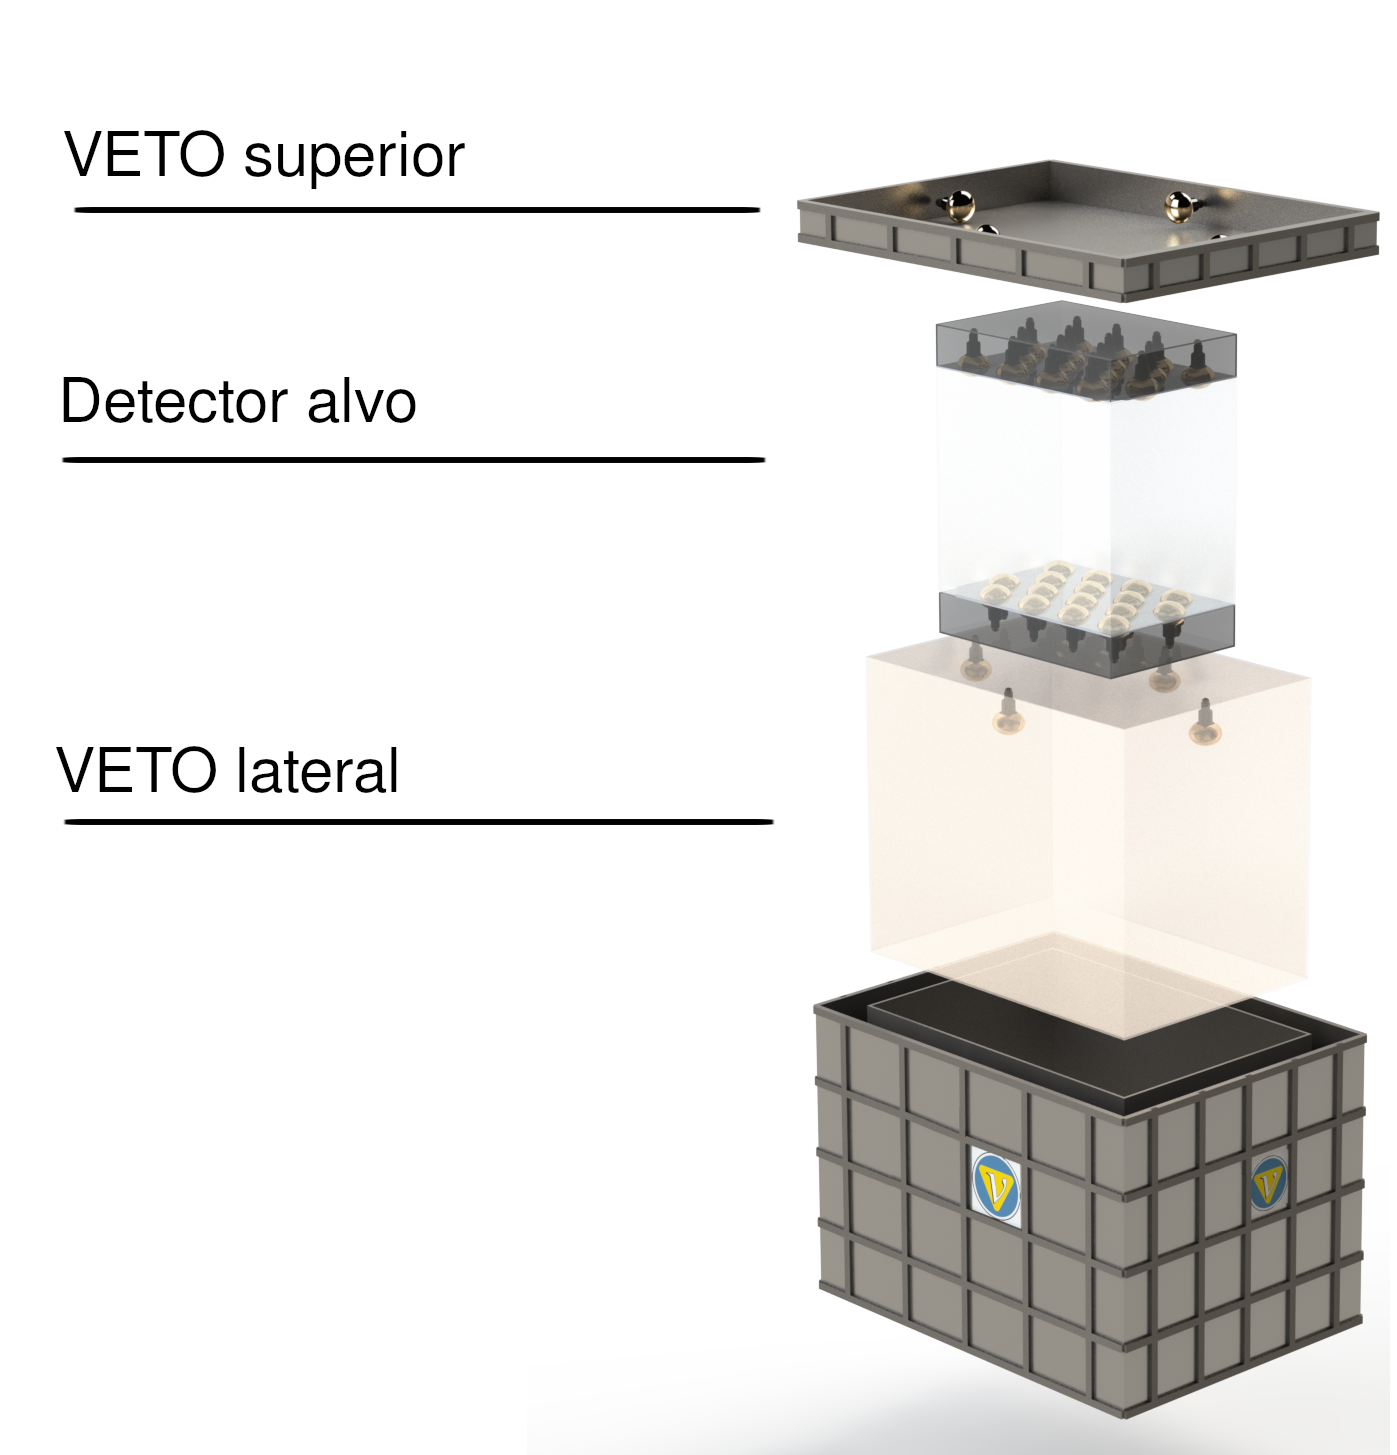
\includegraphics[width=11cm]{textuais/experimento/figuras/detector.png}
    \caption{Vista explodida do detector}
    \label{fig:detector}
\end{figure}

\subsection{Sistemas de \emph{VETO}}

Como o detector $\nu$-Angra é um detector de superfície ele não está imune à radiação advinda do cosmos, se fazendo necessário uma camada de veto para detecção de ruídos de fundo afim de selecionar apenas os eventos de antineutrinos. Cada camada de \emph{VETO} têm 4 PMTs, sendo as do \emph{VETO} superior sendo posicionadas no ponto central de cada aresta, enquanto as do \emph{VETO} lateral ficam na parte superior das faces laterais do detector, somando-se 8 PMTs. O veto lateral é revestido com uma fina camada de aço para bloquear principalmente nêutrons. \url{http://lsd.cbpf.br/doc/dissertacoes/TeseDoutorado_DionRibeiro.2019_05_07.pdf}

\subsection{Detector alvo}

Como eventos de antineutrinos são de baixa energia, para melhor leitura dos eventos, o alvo apresenta 16 PMTs na sua parte inferior e 16 na parte superior, ele é preenchido com um cintilador dopado com gadolínio afim de aumentar o número de partículas livres que interagem com antineutrinos através do processo de decaimento beta-inverso. O detector alvo têm volume aproximado de $1$  m$^3$, e tem a carcaça feita de polipropileno.



\begin{equation}
n \rightarrow p + e^- + \bar{\nu}_e 
\end{equation}

\section{Eletrônicas de \emph{front-end} e aquisição}

Para fazer a aquisição dos sinais das PMTs, o detector dispõe de circuitos eletrônicos para condicionamento dos sinais, chamado de \emph{front-end}, e um sistema de aquisição dos dados, chamado de \ac{NDAQ}. Cada PMT tem uma \emph{front-end} conectada à saída de sinal que então estão ligadas em cada um dos oito canais de cada NDAQ, fazendo-se assim $40$ placas de \emph{front-end} e $5$ NDAQs para a aquisição de todas as PMTs do detector.

Durante todo o tempo os sinais das PMTs são salvos em uma fila do tipo FIFO (do inglês \emph{first in first out}) nas NDAQs, quando um sinal é detectado o conteúdo das \emph{fifos} é esvaziado, digitalizado pelas NDAQs e salvo em um arquivo para análise prévia.


\chapter{Dados Reais} \label{cap:dadosreais}
\vspace{-2cm}

Durante o período de maio a julho de 2017 foram feitas aquisições de dados do detector para raios cósmicos, utilizando duas pás cintiladoras de dimensões $14$x$14$x$1$ posicionadas acima do plano superior do detector como sistema de \emph{trigger}. A primeira pá foi posicionada a $4.5$ cm acima da superfície superior do detector enquanto a segunda pá foi posicionada a $47.5$ cm da mesma superfície.

O sistema de \emph{trigger} foi configurado para realizar a aquisição dos dados das PMTs caso ambas as pás cintiladoras tenham detectado um sinal, fazendo a aquisição dos dados salvos nos \emph{buffers} das NDAQs, salvando as últimas $100$ amostras digitalizadas. Foram selecionados no total $9999$ eventos consecutivos registrados pelo detector para análise deste trabalho.



\section{Metodologia de análise dos dados do experimento}

Os dados do experimento são salvos em arquivos de texto com o valor analógico da saída de cada PMT convertido para um valor digital, valor tal será referido como \emph{ADC counts} a partir deste ponto. Podemos estimar a quantidade de p.e. total por evento estimando a contagem de  \emph{ADC counts} no pico do mesmo, assim, a estratégia para a análise será estimar a quantidade de p.e. por PMT por evento, verificar a quantidade de p.e. por evento e por PMT.

Como no sistema existe uma tensão de \emph{bias} negativa, conhecida como pedestal, precisamos removê-la antes de começar uma análise mais profunda dos dados, centralizando nossas amostras no valor nulo. O pedestal pode ser visto e comparado com uma amostra sem o mesmo na Figura \ref{fig:pedestal}.

\begin{figure}[H]
	\centering
	%	\hspace*{-2cm}
	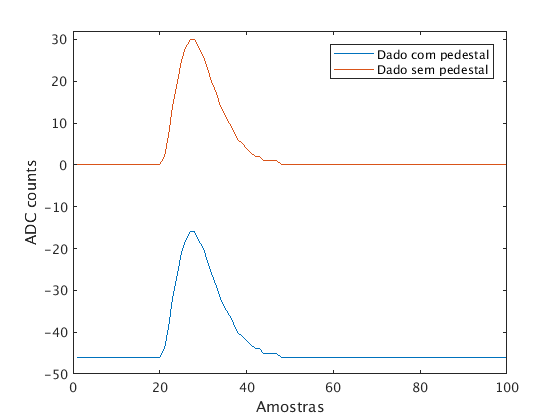
\includegraphics[width=14cm]{textuais/dadosreais/figuras/pedestal.png}
	\caption{Sinal com e sem pedestal}
	\label{fig:pedestal}
\end{figure}

Afim de definir o número de p.e. de cada PMT verificamos o valor máximo de cada PMT. Devido à saturação das PMTs e da eletrônica de \emph{front-end}, os dados coletados com pico de energia acima do valor de saturação devem ser recuperados de alguma forma, foi utilizado um \emph{fitting} com uma forma do sinal conhecida através de um processo iterativo, calculando o erro provável de uma área linear pelo teste do $\chi^2$ (qui-quadrado, Apêndice \ref{apdx:qui-quadrado}) e utilizando a forma final com menor erro, estimando assim, a forma do sinal não saturado. Um exemplo de sinal saturado e sua estimação está presente na FIgura \ref{fig:saturado}.

\begin{figure}[H]
	\centering
%	\hspace*{-2cm}
	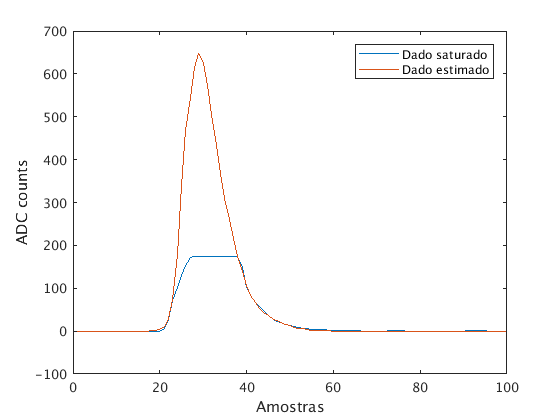
\includegraphics[width=14cm]{textuais/dadosreais/figuras/saturado.png}
	\caption{Sinal de uma PMT saturada versus sua estimação de pico}
	\label{fig:saturado}
\end{figure}

Para verificar as quantidades de p.e. por evento e por PMT, será feito um histograma para cada caso. 

\section{Debug dos dados reais}


Após o \emph{fit} dos dados, foi encontrado um problema intrínseco ao método, como o \emph{fit} era realizado a partir do ponto de saturação eventos naquele ponto foram, em sua maioria, removidos do sistema como pode ser visto no histograma da Figura \ref{fig:peakdist_errado}.

Para resolver este problema precisamos modificar o modo de \emph{fit} a ser realizado. Foi feito então o mesmo método anterior, porém a partir de um ponto em que as PMTs não estão em saturação, mantendo o valor próprio e estimando os valores além de do ponto não saturado, resolvendo o erro de estimação e gerando a Figura \ref{fig:peakdist}.

\begin{figure}[H]
	\centering
%	\hspace*{-2cm}
	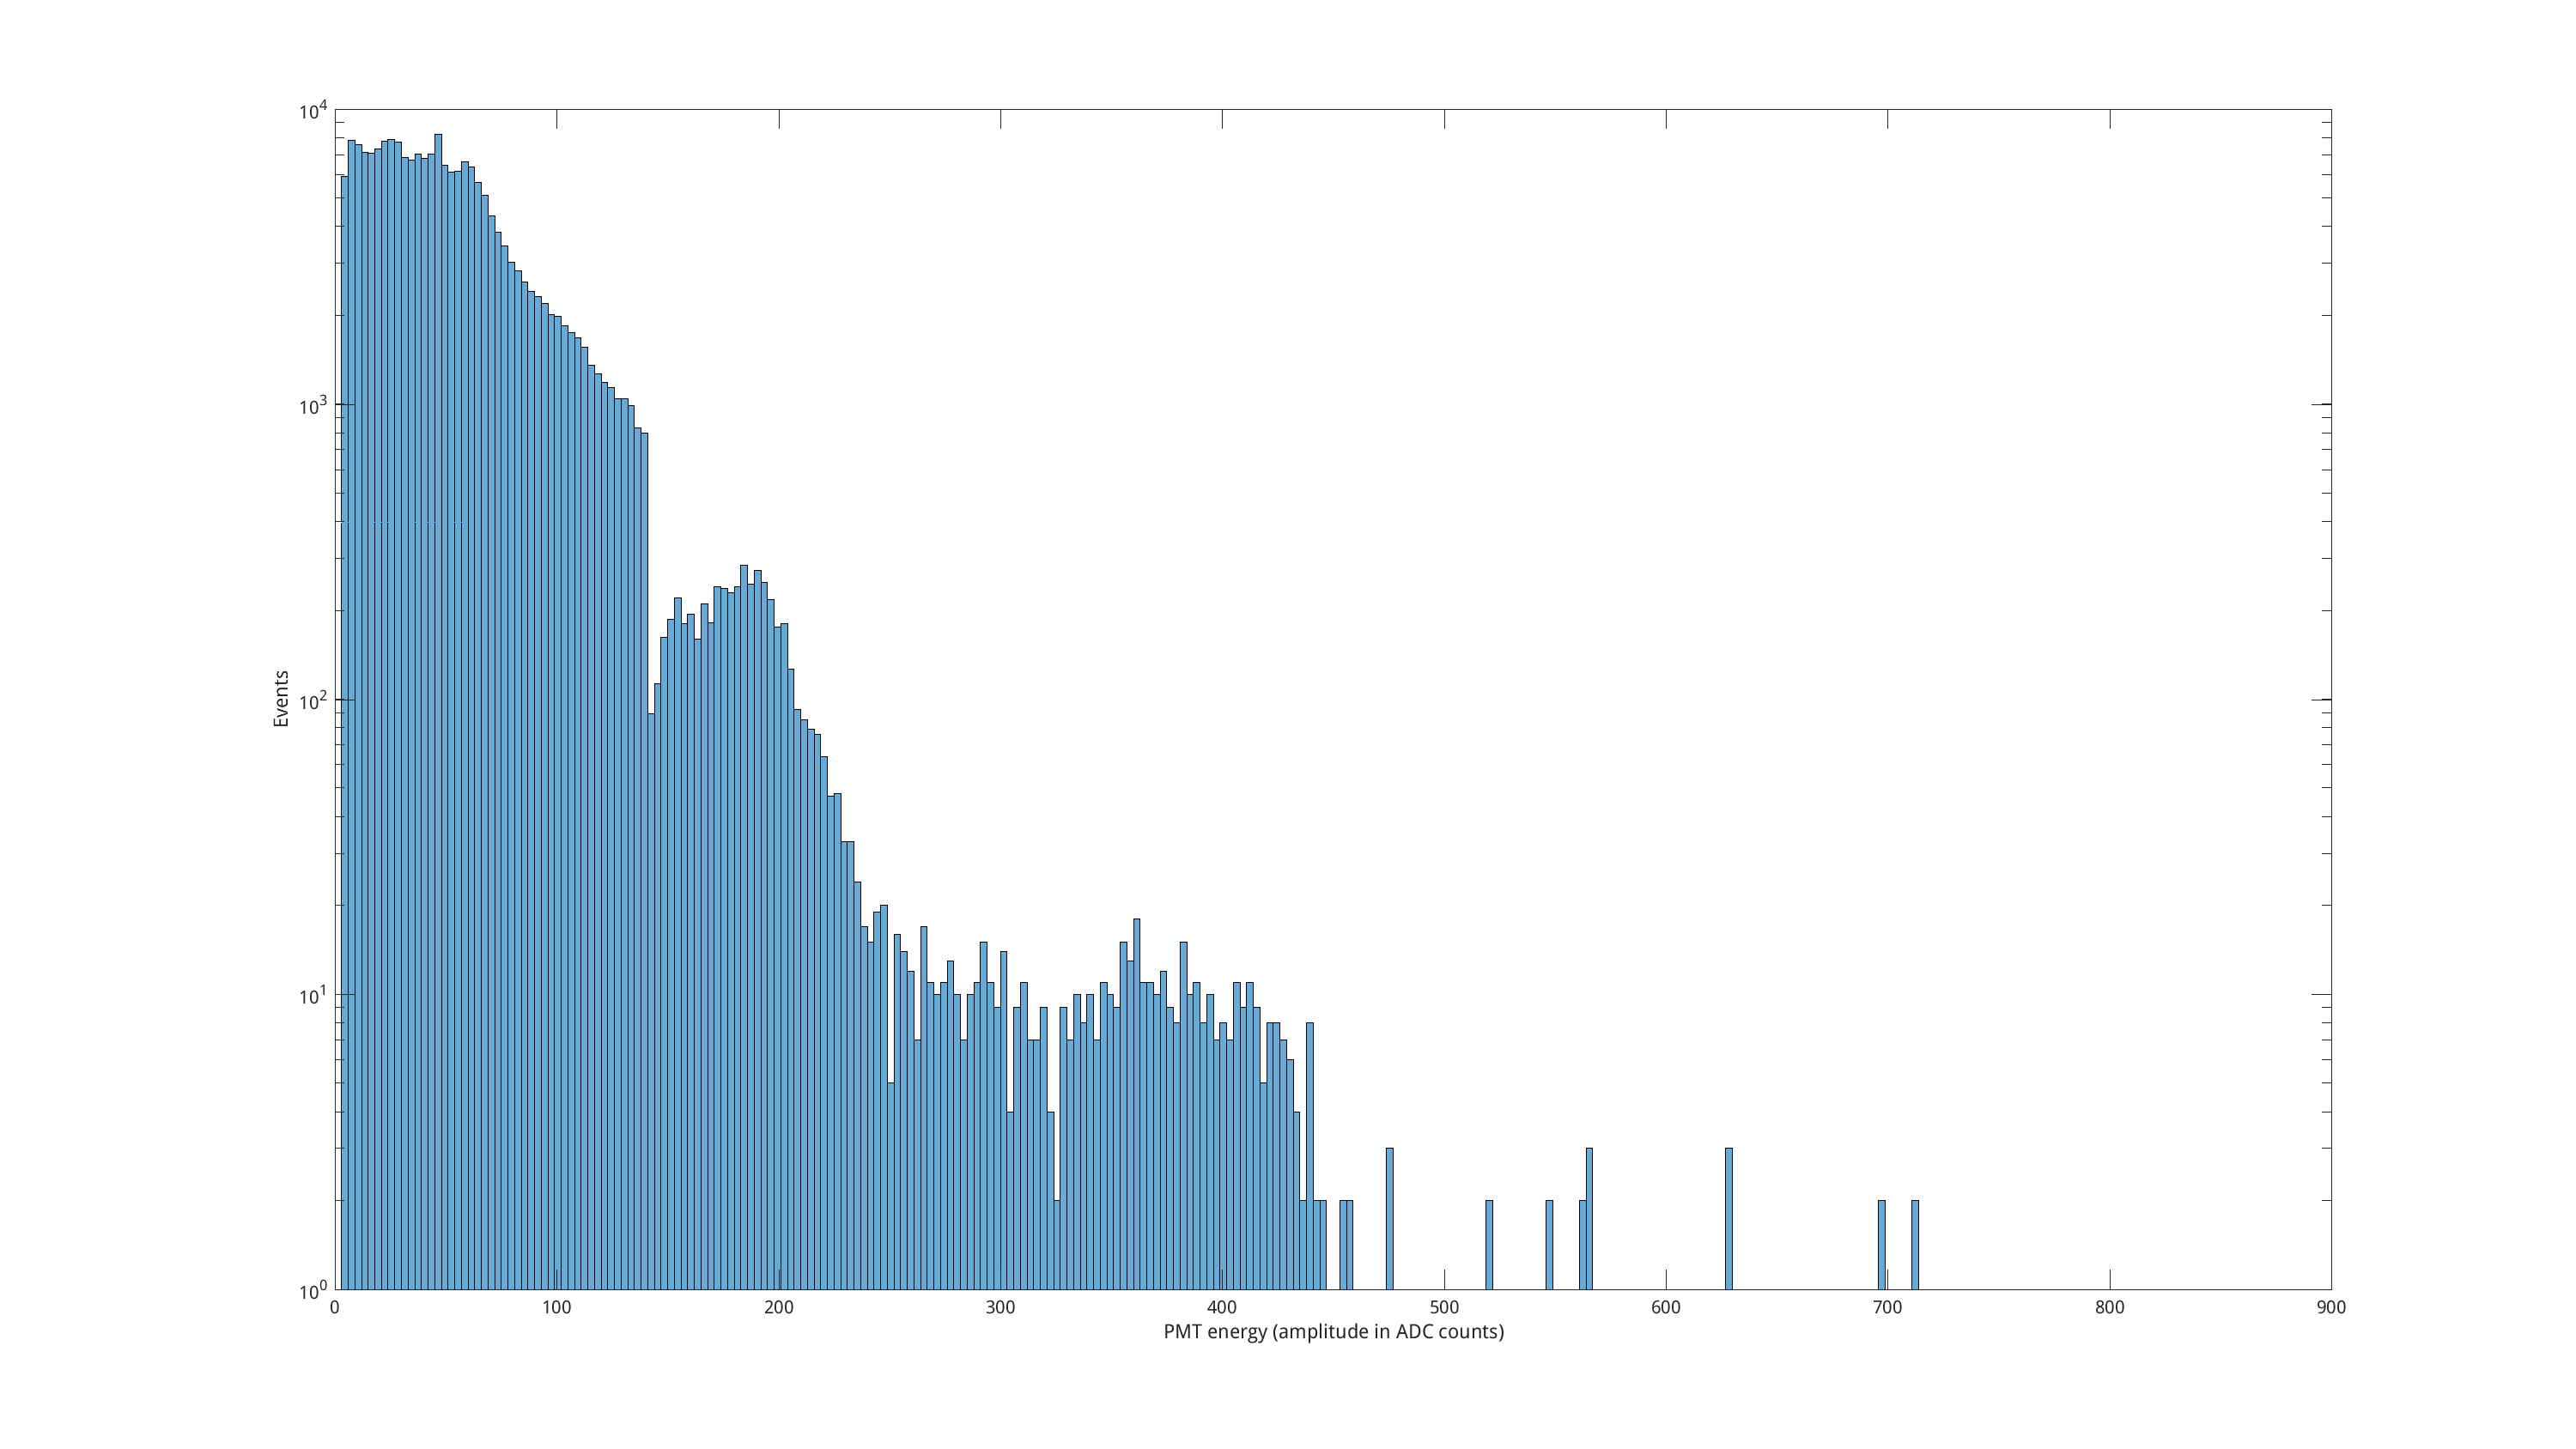
\includegraphics[width=14cm]{textuais/dadosreais/figuras/peakdist_errado.png}
	\caption{Distribuição de picos com problema causado pela estimação}
	\label{fig:peakdist_errado}
\end{figure}

\begin{figure}[H]
	\centering
	%	\hspace*{-2cm}
	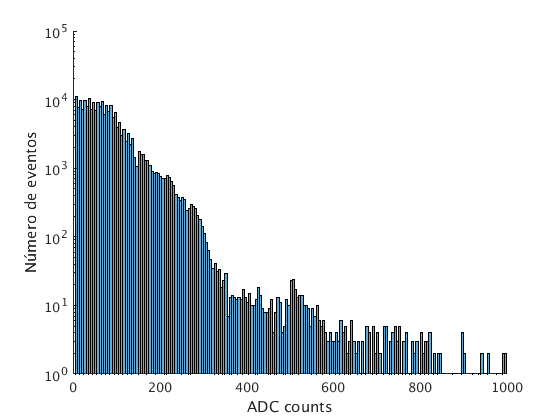
\includegraphics[width=14cm]{textuais/dadosreais/figuras/peakdist.png}
	\caption{Distribuição de picos após a resolução do problema de estimação}
	\label{fig:peakdist}
\end{figure}


\section{Dados da aquisição}

Após resolver os problemas de saturação e estimação dos sinais, temos os dados  a serem comparados com a simulação, representados pelas Figuras \ref{fig:peakdist} e \ref{fig:hist_evt}.

A Figura \ref{fig:hist_evt} representa a quantidade de p.e. por evento, ou seja, a soma de todas as PMTs do detector central, e a Figura \ref{fig:peakdist} representa a distribuição de p.e. para todas as PMTs indivitualmente.
\\

\begin{figure}[H]
	\centering
%	\hspace*{-2cm}
	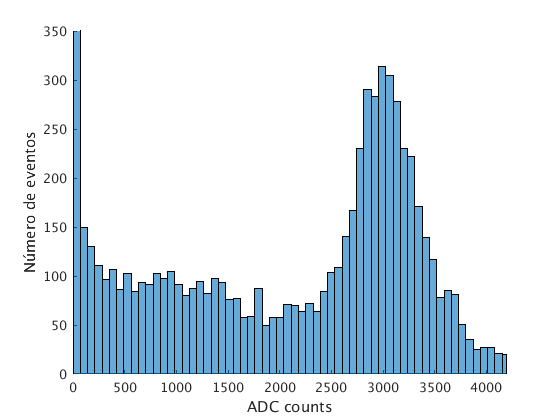
\includegraphics[width=14cm]{textuais/dadosreais/figuras/hist_evt.png}
	\caption{Distribuição de picos após a resolução do problema do \emph{fit}}
	\label{fig:hist_evt}
\end{figure}


\chapter{Simulação} \label{cap:simulacao}
\vspace{-2cm}

Este capítulo será apresentada a plataforma Geant4, interface usada para simulação de eventos ocorridos no experimento $\nu$-Angra com 

\begin{figure}
    \centering
    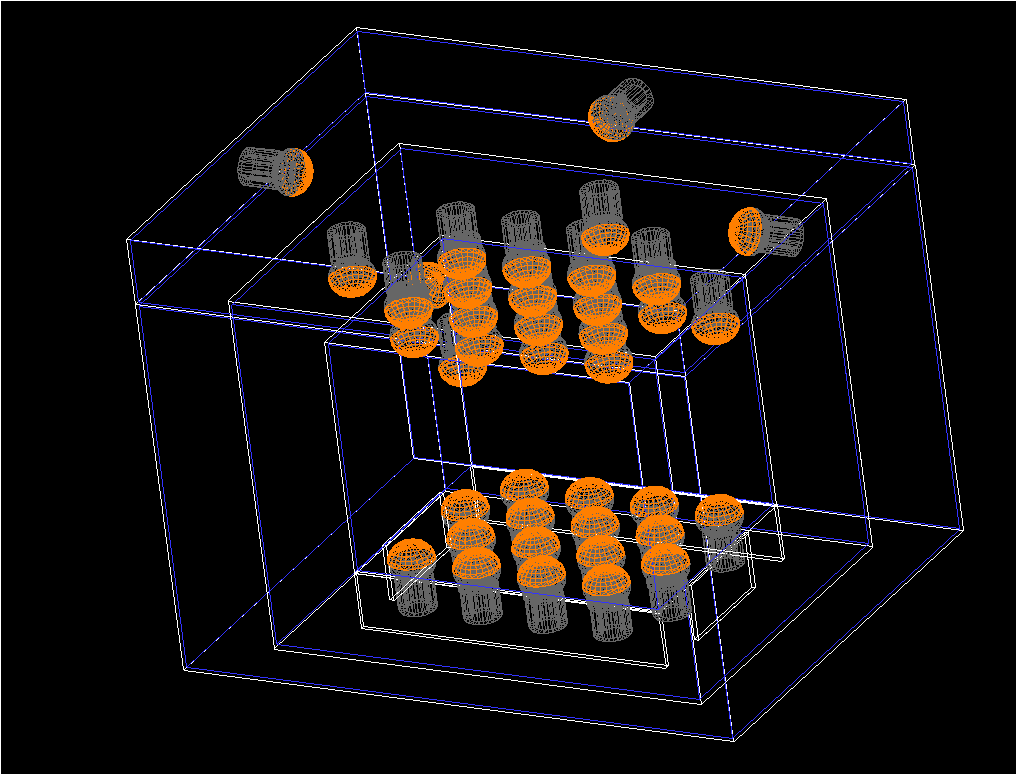
\includegraphics[width=16cm]{textuais/simulacao/figuras/sim_det.png}
    \caption{Detector visto pelo Geant4}
    \label{fig:simdetector}
\end{figure}
\chapter{Resultados} \label{cap:resultados}
\vspace{-2cm}

Após as correções da simulação explicadas no Capítulo \ref{cap:simulacao} Sessão \ref{sec:bugs}, encontramos a qualidade da água $70\%$ pior do que uma água pura. Os histogramas de energia podem ser vistos nas Figuras \ref{fig:a5} e \ref{fig:b4}. A curva de transformação está representada na Figura \ref{fig:transf}.


\begin{figure}[H]
	\centering
	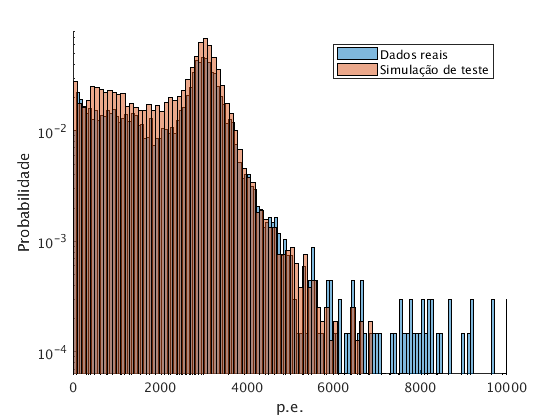
\includegraphics[width=10cm]{textuais/simulacao/figuras/hist_evt4.png}
	\caption{Histograma da energia por eventos com a qualidade da água 70\% pior que a original}
	\label{fig:a5}
\end{figure}

\begin{figure}[H]
	\centering
	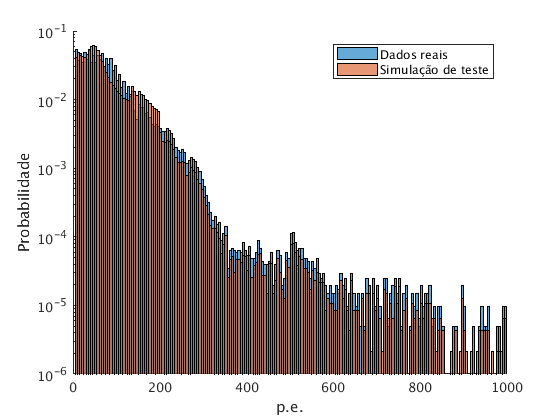
\includegraphics[width=10cm]{textuais/simulacao/figuras/hist_pmt4.png}
	\caption{Histograma da energia por PMT com a qualidade da água 70\% pior que a original}
	\label{fig:b4}
\end{figure}

\begin{figure}[H]
	\centering
	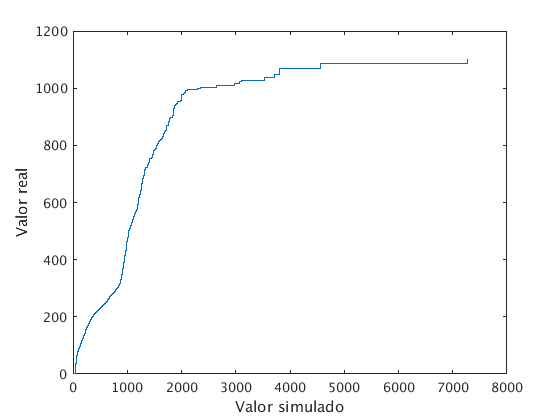
\includegraphics[width=10cm]{textuais/simulacao/figuras/cdfe.png}
	\caption{Transformação de CDFe dos valores simulados para valores reais }
	\label{fig:transf}
\end{figure}


Pôde ser visto uma distorção no histograma de energia por PMT (Figura \ref{fig:b4}) após o método da CDFe, este erro pode ser atribuído à transição de transformação e os valores originais da simulação. Este problema modifica a distribuição (probabilidade) das energias porém mantém o formato da transformação.
\chapter{Conclusão} \label{cap:conclusao}
\vspace{-2cm}

Este trabalho apresentou um estudo e aprimoramento da simulação do experimento $\nu$-Angra. O principal objetivo deste trabalho foi a comparação entre dados simulados e dados reais levando a algumas propostas de correção para o pacote de simulação relacionados à saturação do sistema de leitura do Experimento e ao parâmetro de simulação que ajusta a qualidade da água (caminho livre médio dos fótons). A simulação do experimento $\nu$-Angra ainda se encontra em fase de validação e uma busca por ajustes e/ou erros de implementação ainda devem ser considerados para que a mesma possa ser usado de modo mais conclusivo na processo de entendimento do detector e dos dados experimentais coletados.

\section{Próximos Passos}

Como indicado no Capítulo \ref{cap:simulacao}, a implementação da não-linearidade das PMTs e a saturação da eletrônica podem ser considerados na simulação caso haja interesse em se estudar eventos de mais altas energias (como considerado neste trabalho); a qualidade da água poderia ser medida diretamente e fontes radioativas poderiam ser usadas para fins de calibração do detector, para que se ajuste alguns parâmetros da simulação diminuindo ou até dando fim com a necessidade de se usar uma região mais energética dos eventos adquiridos pelo detector que saturam os canais da \textit{front-end} e das PMTs; pode-se também buscar uma calibração da água através da distribuição do elétron de Michel ao invés do espectro de múons uma vez que este anterior se encontra em uma região de mais baixa energia, com um impacto menor da saturação dos canais de leitura do detector na estimação das energias dos eventos. Deve-se também continuar com afinco a investigar sobre os motivos que levam às diferenças encontradas entre os dados reais e simulados para que seja possível encontrar eventuais erros de implementação, como aquela do vácuo nas PMTs, e, se possível, implementar um sistema \emph{multihreaded} para melhor eficiência computacional do projeto.

%%%%%%%%%%%%%%%%%%%%%%%%%%%%%%%%%
%                               %
%         P\'{o}s textuais          %
%                               %
%%%%%%%%%%%%%%%%%%%%%%%%%%%%%%%%%


\bibliographystyle{abnt-alf}	     % Existem ainda: abbrv,acm,alpha,amsalpha e amsplain
\bibliography{./referencias/bibliografia}  % o nome do arquivo .bib com as refer\^{e}ncias

\appendix

%\include{./postextuais/apendice/apendiceAtlas}
%\include{./postextuais/apendice/apendicePubli}
\chapter{A radiação de Cherenkov}\label{apdx:cherenkov}

Techniques for nuclear and particle physics experiments, a how-to approach - W.R. Leo

A radiação de Cherenkov acontece quando partículas carregadas atravessando um meio têm velocidades maiores que a velocidade da luz naquele meio, ou seja:

\begin{equation}
    v_{partícula} > \dfrac{c}{n}
\end{equation}

onde $c$ é a velocidade da luz no vácuo e $n$ é o índice de refração do meio.

Nestes casos, uma onda de choque eletromagnética é enviada para o meio formando um cone com um ângulo definido 

\begin{equation}
    \cos{\theta_C} = \dfrac{1}{\beta n(\omega)}
\end{equation}

\begin{figure}[H]
    \centering
    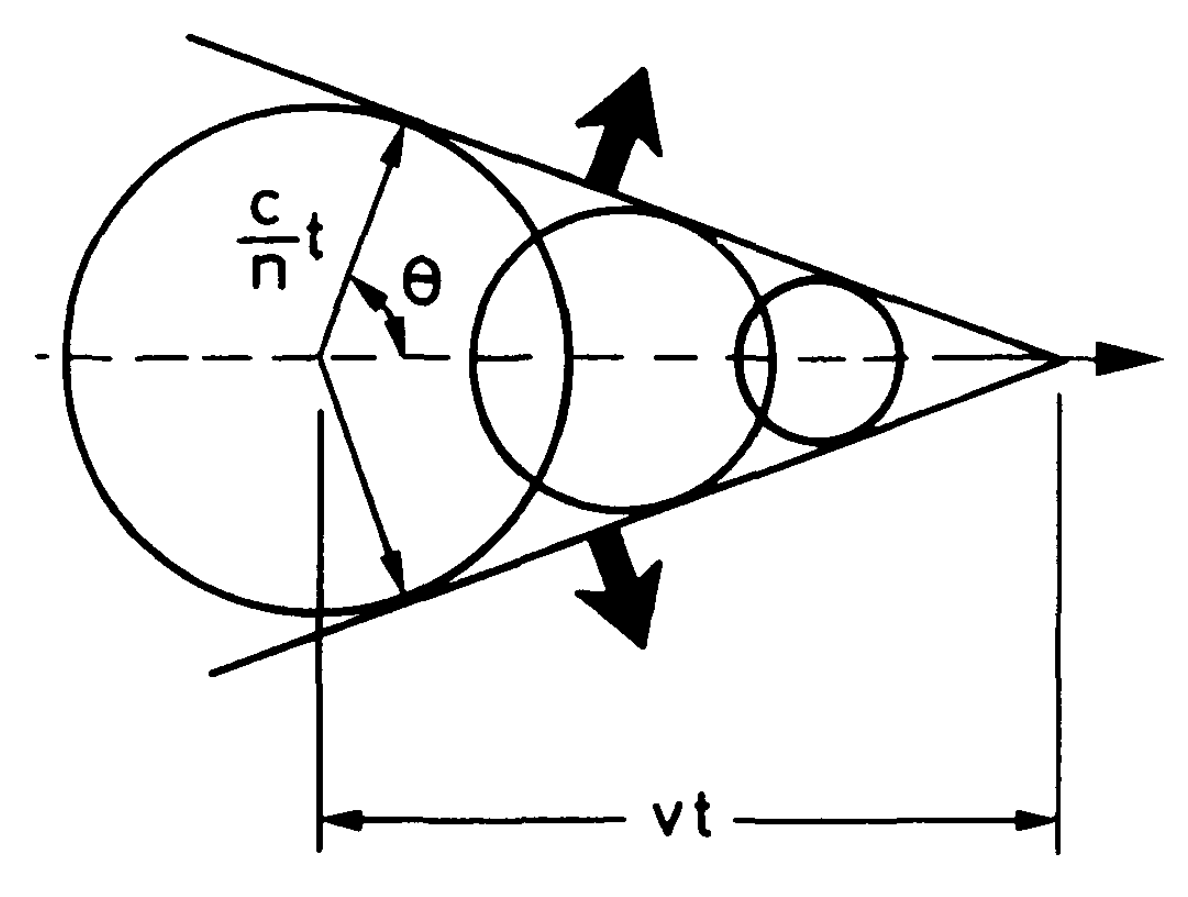
\includegraphics[width=6cm]{postextuais/apendice/figuras/cherenkov.png}
    \caption{Radiação de Cherenkov: uma onda de choque eletromagnética formada pela passagem de partículas acima da velocidade da luz no meio}
    \label{fig:my_label}
\end{figure}

em respeito à trajetória da partícula. A radiação incide em forma de fótons, geralmente no espectro do ultra-violeta, detectáveis por materiais fotosensíveis como PMTs ou \ac{SiPMs}.
\chapter{Qui-quadrado} \label{apdx:qui-quadrado}

Fundamento da teoria de erros - José Henrique Vuolo

Sendo $f(x)$ a função ajustada a um conjunto de $n$ pontos experimentais $(x_i, y_i)$ e o desvio padrão $\sigma$, a quantidade de $\chi^2$-estatístico é definida por

\begin{equation}
\chi^2 = \dfrac{1}{\sigma^2} \sum_{i=1}^{n}[y_i - f(x_i)]^2
\end{equation}

O valor de $\chi^2$ define então o erro estatístico do
%\include{./postextuais/apendice/apendiceB}
%
%\include{/postextuais/apendice/apendiceC}




\end{document}
